
We introduce the software we developed for the power analysis of genetic association studies of qualitative traits in this appendix.
Section \ref{sec:power-analysis-overview} reviews the typical process of study planning employed by geneticists.
Disease models are often used to specify the distribution of observations under the alternative hypothesis in power analysis. 
In Section \ref{sec:disease-models}, we revisit the use of these disease models and argue for an alternative way of model parametrization that is better suited to conducting systematic reviews and confirmatory studies.
Section \ref{sec:user-guide} provides three example usages of the software.
Instructions for downloading, installing, launching, and terminating the software can be found in Section \ref{sec:UPASS-misc}.

\section{Power analysis in genetic association studies}
\label{sec:power-analysis-overview}
We briefly review the main steps of a typical power analysis for genetic association studies.

\medskip
{\bf 1. Disease model specifications.}
A typical power analysis for genetic association studies begin by specifying an alternative hypothesis through a disease model (dominant, recessive, multiplicative, additive, etc.), which assumes:

\begin{itemize}
    \item The genotype relative risks (GRR).
    \item Risk allele frequency in the general population ($p$).
    \item Disease prevalence in the general population (Prev).
\end{itemize}

The disease model and parameters determine the joint distribution of the genotypes and phenotyes {\it in the population}, shown in the following table.

\begin{center}
    \begin{tabular}{cccc}
    \hline
    & \multicolumn{3}{c}{Risk allele copies} \\
    \cline{2-4}
    Population Prob. & 0 copies & 1 copy & 2 copies \\
    \hline
    Cases & $\pi_{10}$ & $\pi_{11}$ & $\pi_{12}$ \\
    Controls & $\pi_{20}$ & $\pi_{21}$ & $\pi_{22}$ \\
    \hline
    \end{tabular}
\end{center}

In the disease models, the conditional probabilities of having the disease, given the risk allele copy numbers, satisfy the following relations,

\begin{equation} \label{eq:GRR}
    \frac{\pi_{10}}{\pi_{10} + \pi_{20}} : \frac{\pi_{11}}{\pi_{11} + \pi_{21}} : \frac{\pi_{12}}{\pi_{12} + \pi_{22}}
    = \begin{cases}
    1 : \text{GRR} : \text{GRR}^2, &\text{Multiplicative} \\
    1 : \text{GRR} : 2\times\text{GRR}-1, & \text{Additive} \\
    1 : \text{GRR} : \text{GRR}, & \text{Dominant} \\
    1 : 1 : \text{GRR}, & \text{Recessive}
\end{cases}
\end{equation}
where GRR is strictly greater than 1 under the alternative, and equal to 1 under the null hypothesis.

The disease prevalence determines the sum of the probabilities of cases in the population,
\begin{equation} \label{eq:prev}
    \pi_{10} + \pi_{11} + \pi_{12} = \text{Prev}.
\end{equation}

The risk allele frequency in the general population, $p$, assuming Hardy-Weinberg equilibrium, satisfies 
\begin{equation} \label{eq:RAF-pop}
    \pi_{10} + \pi_{20} = (1-p)^2, \quad \pi_{11} + \pi_{21} = 2p(1-p), \quad \pi_{12} + \pi_{22} = p^2.
\end{equation}

The population probabilities are determined by the disease model and its parameters (GRR, Prev, and $p$).
The six unknowns  $(\pi_{10},\ldots,\pi_{22})$ and are solved for using the six equations above: two from Relation \eqref{eq:GRR}, one from \eqref{eq:prev}, and three from \eqref{eq:RAF-pop}.


\bigskip
{\bf 2. Sampling adjustments.}
Next, the probabilities of observing each genotype-phenotype combination are adjusted according the number of cases and controls recruited \emph{in the studies}, where the sample sizes are specified with the number of cases ($n_1$) and controls ($n_2$), or equivalently, the fraction of cases ($\phi$) and total number of subjects ($n$).

\begin{center}
    \begin{tabular}{cccc}
    \hline
    & \multicolumn{3}{c}{Risk allele copies} \\
    \cline{2-4}
    Prob. in study & 0 copies & 1 copy & 2 copies \\
    \hline
    Cases & $\pi_{10}\frac{\phi}{\text{Prev}}$ & $\pi_{11}\frac{\phi}{\text{Prev}}$ & $\pi_{12}\frac{\phi}{\text{Prev}}$ \\
    Controls & $\pi_{20}\frac{1-\phi}{1-\text{Prev}}$ & $\pi_{21}\frac{1-\phi}{1-\text{Prev}}$ & $\pi_{22}\frac{1-\phi}{1-\text{Prev}}$ \\
    \hline
    \end{tabular}
\end{center}

As an example, if $\phi > \text{Prev}$, the probabilities are adjusted to account for over-sampling of cases.
Conversely, adjustments are needed to account for under-sampling of cases.

The relative frequencies of allele type-phenotype combinations {\it in the study} are then calculated as follows.

\begin{center}
    \begin{tabular}{ccc}
    \hline
    & \multicolumn{2}{c}{Allele variant} \\
    \cline{2-3}
    Prob. in study & Risk allele & Non-risk allele \\
    \hline
    Cases & $\phi\left(\frac{\pi_{12}}{\text{Prev}}+\frac{\pi_{11}}{2\times\text{Prev}}\right)$ & $\phi\left(\frac{\pi_{11}}{2\times\text{Prev}}+\frac{\pi_{10}}{\text{Prev}}\right)$ \\
    Controls & $(1-\phi)\left(\frac{\pi_{22}}{1-\text{Prev}}+\frac{\pi_{21}}{2(1-\text{Prev})}\right)$ & $(1-\phi)\left(\frac{\pi_{21}}{2(1-\text{Prev})}+\frac{\pi_{20}}{1-\text{Prev}}\right)$ \\
    \hline
    \end{tabular}
\end{center}

This final table corresponds to the probabilities underlying the $2\times2$ multinomial counts that we introduced in Chapter \ref{chap:intro}.
We denote the relative frequencies of allele type-phenotype combinations with $\mu = (\mu_{11}, \mu_{12}, \mu_{21}, \mu_{22})$, as we did in Chapter \ref{chap:GWAS}.

\begin{center}
    \begin{tabular}{cccc}
    \hline
    & \multicolumn{2}{c}{Allele variant} & \\
    \cline{2-3}
    Prob. in study & Risk allele & Non-risk allele & Total by phenotype \\
    \hline
    Cases & $\mu_{11}$ & $\mu_{12}$ & $\phi = \mu_{11} + \mu_{12}$ \\
    Controls & $\mu_{21}$ & $\mu_{22}$ & $1-\phi = \mu_{21} + \mu_{22}$ \\
    \hline
    \end{tabular}
\end{center}

\bigskip
{\bf 3. Power calculations.}
Finally, the power of an statistical test is calculated as the probability of (a correct) rejection, assuming that the data (i.e., tabulated counts of the allele type-phenotype combinations) follow a multinomial or binomial distribution with sample size $2n$, since each individual has a pair of alleles.

These steps form the basis of the calculations implemented in the most existing tools, including the GAS calculator \citep{johnson2017gas}.

Some common association tests include the likelihood ratio test, Pearson's chi-square test, tests of zero slope coefficient in logistic regressions, as well as t-tests for equal proportions.
Although not explicitly stated, the GAS calculator assumes the test of association to be Welch's t-test.
In principal, power analysis has to be tailored to the association test used.
Fortunately, many of these tests are asymptotically equivalent in terms of power \citep{ferguson2017course, gao2019upass}, and results of the power approximation applies to all asymptotically equivalent tests.



% \footnote{Caveat: The final step in the power calculations does not apply to association tests performed directly on the 2-by-3 contingency tables of phenotype-genotype combinations (e.g., the Cochran-Armitage test).Therefore, the GAS calculator should not be used if these tests are to be applied.}.



\section{Specification of alternatives in power analysis}
\label{sec:disease-models}


% \subsection{Two ways to specify alternative hypothesis}

In the power calculations outlined in Section \ref{sec:power-analysis-overview}, the disease models are used to describe the distribution of the data under the alternative hypothesis.
Specifically, they are used to specify the conditional distributions of the allele variants, given the phenotypes.
The probability of observing a risk allele in the control group, known as risk allele frequency (RAF), is defined as follows,
\begin{equation}
    f := \mathbb{P}[\,\text{risk allele}\,|\,\text{control group}\,] 
    = \frac{\mu_{21}}{1-\phi} 
    = \frac{\pi_{22} + \pi_{21}/2}{\pi_{22} + \pi_{21} + \pi_{20}}.
\end{equation}
The risk allele frquency is fully determined by the disease model through the probability table $\mu$. This parametrization was also introduced in \eqref{eq:RAF}.

Similarly, the odds ratio between the two allele variants, 
\begin{equation}
    R:=\frac{\mu_{11}\mu_{22}}{\mu_{12}\mu_{21}} 
    = \frac{(\pi_{12} + \pi_{11}/2)(\pi_{20} + \pi_{21}/2)}{(\pi_{10} + \pi_{11}/2)(\pi_{22} + \pi_{21}/2)},
\end{equation}
is also determined by the disease model and its parameters. See definition in \eqref{eq:odds-ratio}.

In turn, the parameters $(f, R)$, together with the sample sizes $(\phi, n)$, fully describe the distribution of our data under the alternative hypothesis (by determining the probability vector $\mu$ and the sample size $n$).
Power of association tests, therefore, depends on (and only on) the set of ``canonical parameters'':

\begin{itemize}
    \item Risk allele frequency among the controls (f).
    \item Odds ratio (R) of having the defined trait between the two allele variants.
    \item One of the two equivalent ways of parametrizing the sample sizes.
\end{itemize}

\begin{figure}
    \centering
    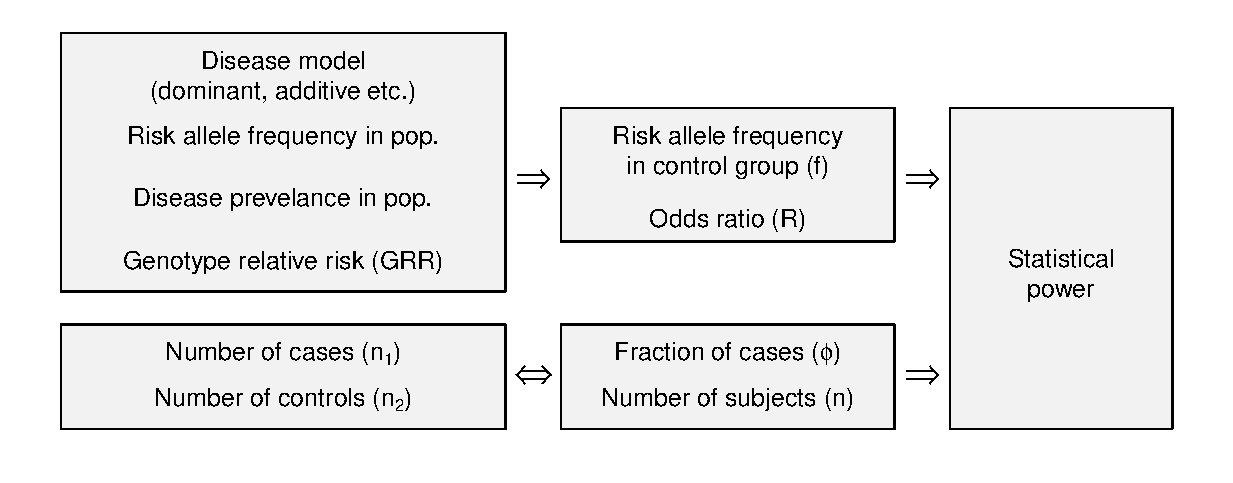
\includegraphics[width=\textwidth]{figures/flowchart.eps}
    \caption{The process of a typical power analysis for genetic association tests.
    The quantities depend on, and can be calculated from the values of their parents in the directed graph. 
    Power can be calculated as long as one set of parameters in each branch is known.
    While there is a one-to-one correspondence between the sample size specifications $(n_1, n_2)$ and $(\phi, n)$, the mapping from disease model specifications to $(f, R)$ is many-to-one. 
    %That is, one cannot recover the disease model specifications from the allelic tables, or equivalently, reported risk allele frequencies and odds ratios.
    }
    \label{fig:flowchart}
\end{figure}

We visualize the process of power analysis in Figure \ref{fig:flowchart}.
Notice that in power calculations, we can either describe the alternative hypothesis with a disease model, or through the canonical parameters ($f, R$). 
Both approaches are sufficient for the purpose of power analysis.
Unfortunately, these two parametrizations are commonly confused.
We emphasize that the risk allele frequency in the control group ($f$) is not equivalent to the risk allele frequency in the general population ($p$); odds ratio ($R$) is not equivalent to genotype relative risk (GRR).

\bigskip

As illustrated in  Figure \ref{fig:flowchart}, power calculations are mediated through the canonical parameters, which are invariant to different model specifications.
That is, different disease model specifications may lead to the {\it same} set of canonical parameters ($f, R$), and consequently the) {\it same} distributions of the allele variant counts.
From a statistical perspective, the disease models that map to the same set of canonical parameters are equivalent in terms of power.

For example, the following set of disease models and parameters imply the same set of canonical parameters $(f = 0.290, R = 1.575)$, and therefore enjoy the same power at the same sample sizes ($n_1 = n_2 = 1000$).
\begin{center}
    \begin{tabular}{cc|cc}
    \hline
    Disease Model & $(\text{Prev}, p, \text{GRR})$ & $(f, R)$ & Power \\
    \hline 
    Multiplicative & $(0.1, 0.3, 1.500)$ & $(0.290, 1.575)$ & 0.990 \\
    Additive & $(0.1, 0.3, 1.588)$ & $(0.290, 1.575)$ & 0.990 \\
    Dominant & $(0.1, 0.3, 1.909)$ & $(0.290, 1.575)$ & 0.990 \\
    Recessive & $(0.1, 0.3, 2.666)$ & $(0.290, 1.575)$ & 0.990 \\
    \hline
    \end{tabular}
\end{center}

Conversely, different disease models with the same parameters, map to drastically different canonical parameters.
For example, the default disease model parameters in the GAS calculator,
\begin{align}
    \text{Disease prevalence in the population}: & \quad \text{Prev} = 0.1 \\
    \text{Risk allele frequency in the population}: & \quad p = 0.5\\
    \text{Genotype relative risk}: & \quad \text{GRR} = 1.5.
\end{align}
map to very different canonical parameters under different disease model assumptions (assuming the same sample sizes of $n_1 = n_2 = 1000$), which leads to drastically different statistical power.
\begin{center}
    \begin{tabular}{cc|cc}
    \hline
    Disease Model & $(\text{Prev}, p, \text{GRR})$ & $(f, R)$ & Power \\
    \hline 
    Multiplicative & $(0.1, 0.5, 1.5)$ & $(0.489, 1.568)$ & 0.995 \\
    Additive & $(0.1, 0.5, 1.5)$ & $(0.491, 1.453)$ & 0.920 \\
    Dominant & $(0.1, 0.5, 1.5)$ & $(0.495, 1.224)$ & 0.282 \\
    Recessive & $(0.1, 0.5, 1.5)$ & $(0.494, 1.281)$ & 0.098 \\
    \hline
    \end{tabular}
\end{center}

In the application, we provide users with a ``Disease model converter'' that implements this many-to-one conversion from the disease model specifications to the canonical parameters.


% \subsection{Comparisons of the two approaches}
% \label{subsec:comparing-two-approaches}
\bigskip

While the disease models may carry additional insights into the biological process, the canonical parameters also have their unique advantages.
We offer an incomplete list of comparisons of the two approaches, and discuss their usage in practice.

\medskip\noindent
{\bf Interpretability and communicability.}
In general, geneticists and biostatisticians seem to agree that disease models are more interpretable.
The concept of genotype relative risks, in particular, seems easier to reason about than odds ratios in the canonical parameters definition.
Disease models also seem to be the de facto mode of model specification when performing power analysis for study planning and grant applications.

The ``nonparametric'' approach to model specification through the canonical parameters is somewhat lesser known to the statistical genetics community.
The canonical parameters are typically estimated and reported as outcomes of the research, but not used as inputs to the power analysis for planning purposes.

\medskip\noindent
{\bf Availability of parameter estimates.}
The canonical parameters $f$ and $R$ can be estimated from data collected in the study.
They are also reported and curated in GWAS catalogs such as the NHGRI-EBI Catalog \citep{macarthur2016new}.

On the other hand, accurate information regarding the disease model parameters can be more difficult to obtain, partly because some parameters in the disease models cannot be estimated from the association studies alone.

In particular, disease prevalence in population (Prev), as well as risk allele frequency in population ($p$), must be obtained from other studies or surveys targeting the general population; the association studies, unless matching the proportion of cases in the population vs in the study ($\phi=\text{Prev}$), cannot produce estimates without using external information.
Genetic association studies rarely explicitly estimate the disease model and its parameters.
In fact, we are not aware of a GWAS catalog that reports and curates the disease models and their estimated parameters.

This paucity of information on disease model parameters is not an issue if we are planning to study a trait for which we have little prior knowledge.
In this case, the purpose of power analysis is to determine the range of models and parameters that lead to discovery of associations, given the study designs.

In contrast, in confirmatory / follow-up studies and systematic reviews, our main interest is in the statistical validity of the reported findings.
Power analysis then serves to find efficient designs, and to validate the claims made.
Knowledge obtained in prior studies (in the form of parameter estimates) are indeed necessary.

\medskip\noindent
{\bf Robustness against model misspecification.}
Disease models are useful in as much as they help us understand the biology behind the data we observe.
Unfortunately, like all models, they can be misspecified. 
For example, the following genotype relative risks,
\begin{equation*}
    \frac{\pi_{10}}{\pi_{10} + \pi_{20}} : \frac{\pi_{11}}{\pi_{11} + \pi_{21}} : \frac{\pi_{12}}{\pi_{12} + \pi_{22}}
    = 1 : 3 : 4,
\end{equation*}
does not follow any of the common disease models.
In this case, different studies may come up with different disease models (say, Dominant and Additive), and of course, different parameter estimates.

Suppose a researcher wishes to perform a meta analysis or confirmatory experiment of the existing results, where the literature reports inconsistent estimates of disease models and parameters,
he would a have a difficult time pooling the information from these different sources. 
And even when they are pooled, the resulting model usually does not fall in one of the familiar categories --- there is no existing tool with which to perform power analysis.
The researcher will likely have to forgo the information from one model, and use estimates from only the other.

On the other hand, the canonical parameters are invariant to the disease model choices, and accommodate models falling outside the usual categories. 
They can also be easily combined to produce pooled estimates.
This universality allows us to perform power analysis in a unified fashion, regardless of the disease models assumed.
This also paves the way for the ``OR-RAF diagram'', as well as systematic reviews of statistical validity of existing studies; see Section \ref{sec:review-GWAS-studies} below.

\medskip\noindent
{\bf Robustness against human errors.}
The disparity in availability of parameter estimates we mentioned earlier can lead to unintended consequences, one of which is potentially incorrect usage of power calculators.
This issue, although minor, is critical to the correctness of the results of our power analysis.

Recall that the specification of a disease model requires as input the risk allele frequency (RAF) in the general population ($p$).
The RAF reported in the NHGRI-EBI Catalog \citep{macarthur2016new}, in contrast, refers to RAF in the control group ($f$).
With RAF in population often unavailable, it is tempting to substitute the RAF in control group into the calculations.
While the two quantities may be close when diseases prevalence and penetrance are low, their difference becomes non-negligible if either of the two conditions are violated, leading to grossly distorted results.

Performing power analysis with the canonical parameters is not guaranteed to prevent this human error, as mistake in the other direction could also happen.
But perhaps it is more robust to such mistakes, since what is readily available matches with what is required as input.

\medskip\noindent
{\bf Compatibility of parameters.}
We make another minor comment regarding correct usage of disease models.

We caution users that not all values of the disease model parameter combinations are valid.
For example, in a multiplicative model, the parameters 
\begin{equation*}
    p = 0.1, \quad \text{Prev} = 0.5, \quad \text{GRR} = 1.5,
\end{equation*}
would result in the conditional probability of having two risk allele copies greater than 1.
(In this case, the GAS calculator \citep{johnson2017gas} would produce the error message: ``I don't like the genetic model you requested!'', without explicitly pointing to the compatibility issue.)

Although an experienced geneticist would immediately notice the impossibility of the disease model parameter combinations, these contradictions may not be obvious to the untrained eye.
The end user of the software -- experienced or not -- is ultimately responsible for inputting valid values when specifying a disease model.

On the other hand, any combination of 
\begin{equation*}
    f\in(0,1), \quad \text{and} \quad R\in(0,+\infty)
\end{equation*}
is valid. 
Parameter compatibility is not an problem for the set of canonical parameters.

\medskip\noindent
{\bf Recommendations on model specification in power analysis.}
Since both the disease models and the canonical parameters are sufficient for the purpose of power analysis, it is natural to ask why (and when) should one take the canonical parameters approach, given that the more familiar disease models would also suffice.

We believe that either approach may be preferred, depending on the use cases.
Recall that power analysis is useful in at least three scenarios:
\begin{enumerate}
    \item {\it Planning for an exploratory study, where little is known about the associations.}
    
    In this case, the top branch in Figure \ref{fig:flowchart} is unknown to the researcher.
    The goal is to find out the range of disease models and parameters that are discoverable given the study designs.
    Power analysis is also to some extent exploratory in nature.
    
    \item {\it Planning for a confirmatory study, where something is known about the associations and one wishes to validate the findings with an efficient design.}
    
    In this case, the top branch in Figure \ref{fig:flowchart} is known, and the variables in the bottom branch is what we are solving for.
    The goal of power analysis is to provide a set of efficient study designs with sufficient power.
    
    \item {\it Reviewing the reported findings and verify the statistical validity.}
    
    In the third case, one looks to find out whether the claims of statistical significance are congruent with the evidence from data.
    A claim supported by very weak or contradictory evidence should invite further investigations.
    In this case, both branches in Figure \ref{fig:flowchart} have to be available.
\end{enumerate}

In view of the discussions above, we propose the following general guidelines for power analysis in genetic association studies.

\begin{itemize}
    \item When designing an association study where little to no prior information is available, either approach is valid. However, disease models may be easier to interpret and communicate.
    \item When designing a follow-up or confirmatory study, or conducting a systematic review, researchers may wish to choose the approach for which the parameter estimates are available, or of better quality. Typically the canonical parameters are better estimated, reported, and curated.
\end{itemize}
% The simple answer is the following: the canonical parameter approach is better suited to planning confirmatory studies and performing systematic reviews, which to the best of our knowledge, could not be readily done prior to our tool. 
% We expect many exceptions to these suggested choices.
The comments we made about the two approaches should not be taken as criticisms, but rather as reminders of the potential pitfalls in power analysis.
In either approach, care needs to be exercised in order to produce valid results.



\section{Use case illustrations}
\label{sec:user-guide}

The software has three main functionalities, namely, reviewing the GWAS literature, designing prospective association studies, and converting between disease models and canonical parametrizations.
We detail each of the three functionalities of the application, and illustrate with examples.

\subsection{Reviewing reported findings in the GWAS catalog}
\label{sec:review-GWAS-studies}

The ``OR-RAF power diagram'' tab of the application provides a tool for reviewing reported associations from existing studies.
The application calculates statistical power based the core parameters common to models of qualitative traits:

\begin{itemize}
    \item Sample sizes, i.e., the number of cases and controls i.e., $(n_1, n_2)$ or $(\phi, n)$.
    \item The canonical parameters $(f, R)$.
\end{itemize}

Users need only prescribe the sample sizes, by one of two ways provided in the first box, i.e., total sample size + fraction of cases, or number of cases + number of controls.

Statistical power of common association tests, including the likelihood ratio test, chi-square test, Welch's t-test, and the LR test, have the same asymptotic power curves.
This shared power limit is calculated as a function of $f$ and $R$, and visualized as a heatmap referred to as the OR-RAF diagram. 


\bigskip

We provide users the options to load and overlay findings reported in the NHGRI-EBI GWAS Catalog \citep{macarthur2016new}, or upload data from other sources compliant with the Catalog's data format.

The visualization is adaptive and fully interactive.
The initial sample sizes are dynamically adjusted, and automatically determined from texts of the article reporting the user selected loci.
Since the sampling structures are many and varied across different studies, and no uniform reporting format is enforced in the catalog, the initial sample sizes are best estimates from the extracted texts.
Information of the selected loci and the study is also dynamically displayed below the diagram.


\bigskip


The unified power analysis allows us to examine results from different studies employing different models and applicable tests, in the same diagram, with the same power limits.
This allows for a systematic review of reported findings for their statistical validity.
In particular, a reported association predicted to have low power given the study's sample size -- lying in the dark regions of the OR-RAF diagram -- while not impossible, invites further scrutiny.
%\footnote{It should be noted that a reported association predicted to have high power is not automatically accurate, as survival bias induced by multiple testing may inflate the reported $f$ and $R$ estimates.}. 
Studies where reported associations show misalignment with the predicted powered curves should also be further investigated for potential problems in the data curation process.

\begin{figure}
    \centering
    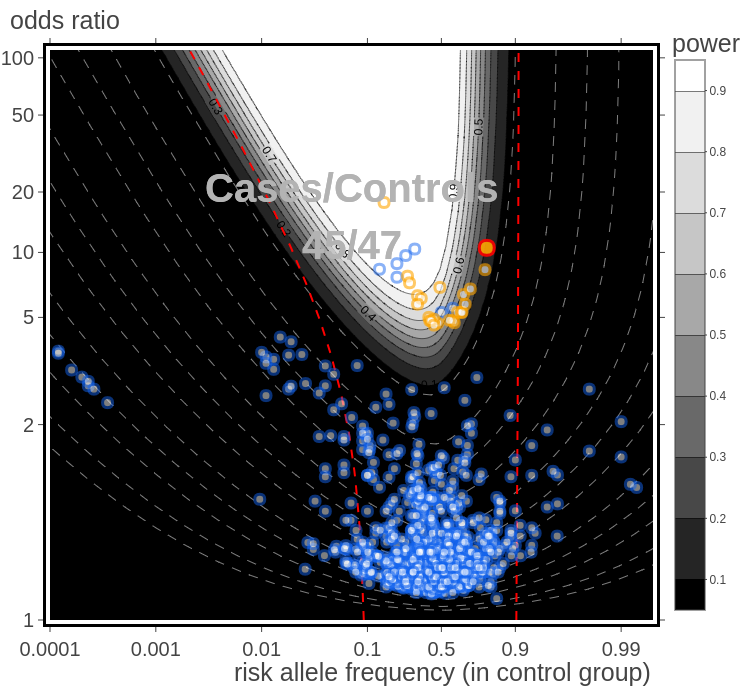
\includegraphics[width=0.49\textwidth]{figures/forensics1.png}
    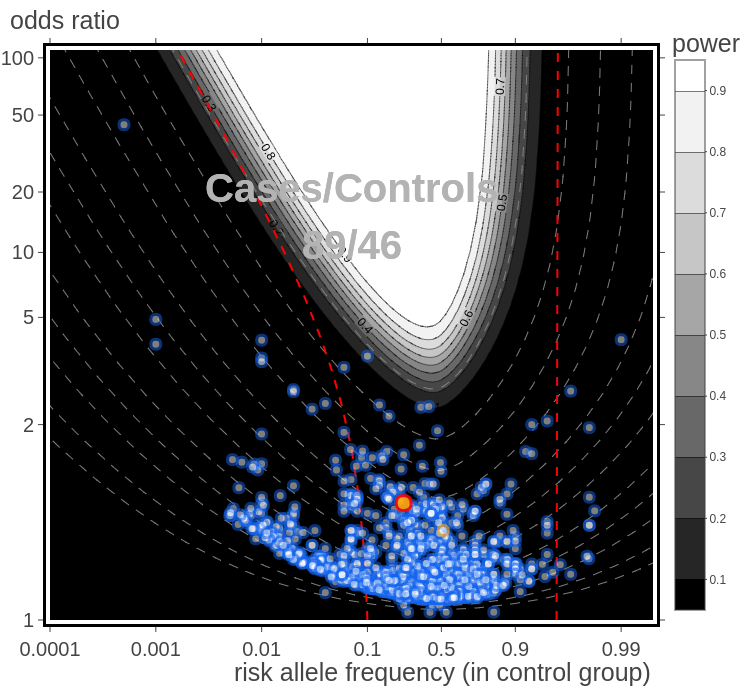
\includegraphics[width=0.49\textwidth]{figures/forensics2.png}
    \caption{The OR-RAF diagram of two studies where gross misalignments were identified. 
    Left: Dominguez-Cruz et al. (2018), right: Haryono et al. (2015). 
    The reported odds ratios and risk allele frequencies of the discovered associations in these two papers are charted with orange (and red) circles. 
    Dark regions represent $f$-$R$ parameter combinations that are predicted to have low power of dicovery under the current sample sizes.
    See text for more comments.}
    \label{fig:forensics}
\end{figure}

We illustrate this forensics feature of the the software with two GWAS studies by \cite{dominguez2018pilot} and \cite{haryono2015pilot}, shown in Figure \ref{fig:forensics}. 
Gross misalignments with our power analysis were identified in both cases.
    Uppon contact, \cite{dominguez2018pilot} confirmed that this misalignment is the result of a problem in the data curation process of the GWAS Catalog (Dominguez-Cruz, personal communication). 
    In particular, the risk allele frequencies reported in the Catalog were based on all subjects in the study, as opposed to only the control group, while the Catalog requires that risk allele frequencies be reported in the control group only. 
    As a consequence, the risk allele frequencies are systematically overestimated, shifting the reported findings to the right in the diagram.
    The study by \cite{haryono2015pilot}, though may very well hold valid results, calls for further scrutiny of its statistical methodologies given the apparent incongruity of its conclusions at the reported the sample sizes.

In general, however, we expect the forensics aspect of our software to be useful for discovering problems with data entry and catalog curation process, as well as for assessing the reproducibility and robustness of reported findings.


\subsection{Designing association studies}
\label{sec:design-my-study}

The ``Design my studies'' tab of the application provides a tool for finding optimal designs of association studies.
The tool requires inputs in a four-step process.
\begin{enumerate}
    \item Model specification.
    \item Sample size constraints specification.
    \item False discovery Criteria specification.
    \item Power specification.
\end{enumerate}
Each of the steps can be specified in a number of alternative ways.

\bigskip
\noindent
{\bf Step 1: Model specification.}
We provide two three ways to describe the model for biological process of the disease or trait of interest.

The distribution of observations can be specified through the canonical parameters, risk allele frequency in the control group ($f$) and odds ratio ($R$).
Estimates for these quantities in previous studies of the same trait can be found in GWAS catalogs such as the NHGRI-EBI Catalog.
See Section \ref{sec:optimal-design} for their definitions.

Alternatively, users may opt to specify through the disease models, of which we implement the four most popular ones: additive, multiplicative, dominant, and recessive.
See Section \ref{sec:power-analysis-overview} below for the definitions of the quantities involved in the disease models.
We remind users the difference between the risk allele frequency in the control group ($f$) versus risk allele frequency in the general population ($p$); only the latter is used in the disease model specifications.

Advanced users may choose to use a more succinct ``signal size per sample'' option, which directly parametrizes the signal sizes ($\lambda/n$).
Definition of signal size $\lambda$ can be found in Section \ref{sec:odds-and-power}.

\bigskip
\noindent
{\bf Step 2: Sample size specifications.}
The second step requires users input the sample size constraints of the study.
The three available options are ``Budget / total number of subjects'', ``Number of cases'', and ``Fraction of cases''.
In the subsequent calculations, the selected and specified quantities are treated as fixed.
With only one unknown parameter left in the flow of power calculations (recall the flowchart in Fig. \ref{fig:flowchart}), we calculate power as a function of the  remaining specified parameter.
In particular,

\begin{itemize}
    \item If the constraint is total budget, power is shown as a function of the fraction of cases.
    \item If the constraint is number of cases, power is shown as a function of the number of controls.
    \item If the constraint is fraction of cases, power is shown as a function of the total number of subjects.
\end{itemize}

\bigskip
\noindent
{\bf Steps 3 and 4: False discovery and power specifications.}
The final two steps require as input the desired level of false discovery and false non-discovery control.
Both specification can be done through the marginal levels, i.e., Type I error and Type II error, or alternatively, through the multiple testing-adjusted levels, i.e., family-wise error rate (FWER) and family-wise non-discovery rate (FWNR).

\begin{figure}
    \centering
    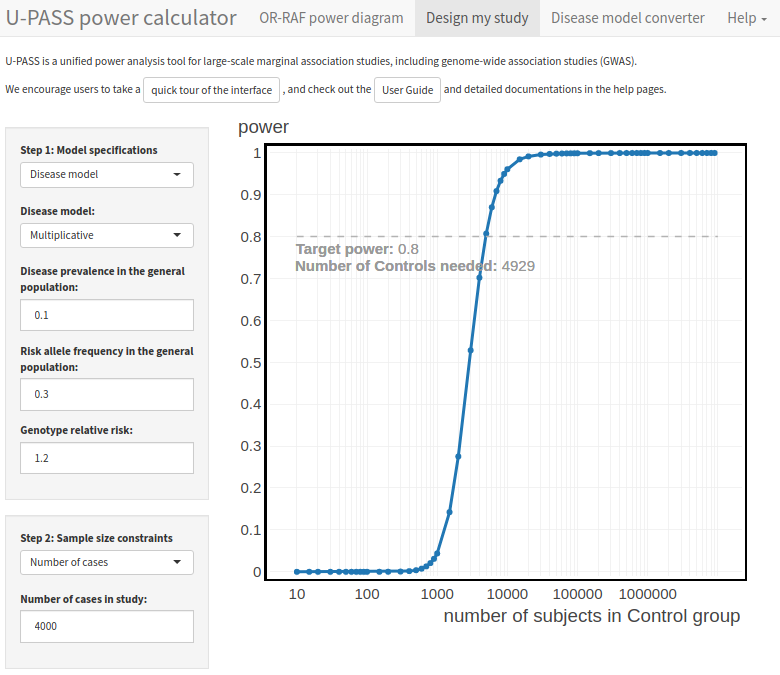
\includegraphics[width=0.8\textwidth]{figures/UPASS_power_analysis.png}
    \caption{A screenshot of the user interface for the ``Design my study'' tab of the software. The inputs are as described in the numerical example in Section \ref{sec:design-my-study}. Results of the power calculation are visualized in an interactive plot in the application.}
    \label{fig:UPASS-power-analysis}
\end{figure}


\bigskip
\noindent
{\bf An example: designing prospective studies.}
A researcher wishes to find out how many controls are needed in order to detect an association between a risk variant described by a multiplicative model with parameters:
$$
\text{GRR} = 1.2, \quad p = 0.3, \quad \text{Prev} = 0.1.
$$
The study has recruited 1000 subjects in the case group, and is aiming for power of 80\% with FWER controlled at 5\% level adjusted for the multiplicity of $10^6$ tests.

In the application, we input the disease model parameters in the first step.
In the second step, we select the sample size constraint as ``number of cases'' and set to 1000.
The third step, we selected FWER as the criteria, and set the appropriate levels and multiplicity; a p-value cut off ($0.05/10^6=5\times10^{-8}$) is automatically calculated and displayed.
The final step, we choose ``Type II error / (1-power)'' as the target and select $1-80\%=20\%$.

The result of the calculation shows that the targeted power cannot be achieved at the current number of cases, no matter how many controls are recruited.
Therefore, the researcher should consider recruiting more subjects in the case group in order to in crease power.
For example, if there are instead 4000 subjects in the case group, then we would need only roughly 4929 controls in order to achieve the desired level of power.


\subsection{Converting disease models into canonical parametrization}

The ``Disease model converter'' tab of the application provides a tool for converting disease models into their implied canonical parameters.
See Figure \ref{fig:UPASS-model-converter} for a screenshot.

\begin{figure}
    \centering
    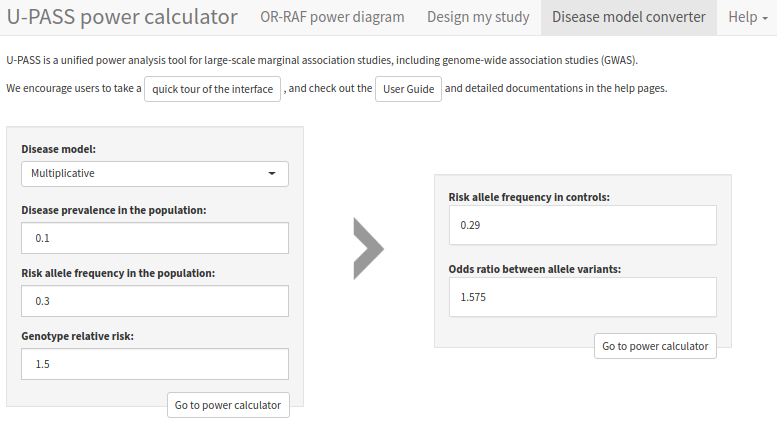
\includegraphics[width=0.8\textwidth]{figures/UPASS_model_converter.png}
    \caption{A screenshot of the user interface for the ``Disease model converter'' tab of the software. See Section \ref{sec:disease-models} for details of the conversion between disease models and canonical parameters in genome-wide association studies.}
    \label{fig:UPASS-model-converter}
\end{figure}

The converter implements the mapping from disease models to the canonical parameters as detailed in Section \ref{sec:disease-models} and  illustrated in Figure \ref{fig:flowchart}.
The tool also allows users to copy the model parameters into the ``Design my study'' tab for power calculations.
Several numerical examples, discussed in Section  \ref{sec:disease-models}, are provided in the tool. 



\section{Download, installation, and usage}
\label{sec:UPASS-misc}
{\bf Software availability.}
U-PASS runs as an R Shiny application. It is a free, open source software under the MIT license.
A live instance of the application is hosted at 
\url{https://power.stat.lsa.umich.edu/u-pass/}.
The source code can be obtained from the repository hosting service Github, by running in the computer's terminal:
\begin{verbatim}
  clone https://github.com/Pill-GZ/U-PASS.git
\end{verbatim}
or by downloading directly from the GitHub page: 
\url{https://github.com/Pill-GZ/U-PASS}.

Should the user choose to run the application from their local machine, we recommend downloading the source code, and follow the next two steps of this user guide.

\bigskip
\noindent
{\bf Installation and dependencies.}
We have collected the required R packages inside the R script
\texttt{install\_required\_packages.R}.
These packages can be installed by navigating to the project folder, and running in the computer's terminal:
\begin{verbatim}
  Rscript install_required_packages.R 
\end{verbatim}
or by running the following command from inside R (RStudio):
\begin{verbatim}
  source("install_required_packages.R")    
\end{verbatim}
The U-PASS software itself requries no installation.

\bigskip
\noindent
{\bf Start/terminate the application.}
The application can be started by running in the computer's terminal:
\begin{verbatim}
  Rscript -e 'library(methods);
              shiny::runApp("./", launch.browser=TRUE)'
\end{verbatim}
or by running the following command from inside R (RStudio):
\begin{verbatim}
  shiny::runApp()
\end{verbatim}
The application can be terminated by simply closing the browser (or browser tab).
Alternatively, the application can be terminated by pressing \texttt{Ctrl} + \texttt{C} in the terminal, or by clicking on the red stop button in Rstudio.

